\section[MIDI: An Introduction]{MIDI}\label{section:midi}

\subsection[What is MIDI?]{What is MIDI?}\label{section:what-midi}
The Musical Instrument Digital Interface (more commonly known as MIDI) is a digital communications protocol which allows for multiple hardware and software electronic instruments, controllers, computers, and related devices to communicate over a connected network\cite{Huber_2012}. It is used most to translate performance \say{events} (or musical notes) into its equivalent digital message, and then transmit these messages to other MIDI devices. These devices (MIDI receivers) can control sound generators or performance generators to create or modify music. Any MIDI-compatible device can send or receive MIDI messages from a MIDI controller (or the device sending the MIDI messages), and this will include all types of synthesizers. As an \say{interface}, MIDI is composed of a data communications link, and a system of hardware and software connected through this MIDI network. With MIDI, any electronic instruments and devices which are within a network can be worked with, through the transmission of a real-time performance and MIDI messages. These transmissions of performances and messages can then be put through the system to various instruments and devices through one singular data line, rather than multiple data streams, as this system can be chained from one device to another. A single data cable used with MIDI is capable of transmitting a real-time performance and MIDI-control message over 16 distinct channels, numbered appropriately one through sixteen. The musician working with the system will determine which of these channels to send information through, depending on which MIDI devices are being used\cite{Romano_2003}.

However, are several limitations to the MIDI protocol. The first, and most important, limitation of MIDI is that it does not support sound. It is unable to communicate audio itself, or create sounds\cite{Huber_2012}. Instead, as a digital language, it instructs a compatible device or program to create, playback, or modify sounds. It will communication an on/off status of a sound trigger, along with a range of parameters which instructs a MIDI receiver to control specified audio-related functions \cite{Kirk_Hunt_2013}. So, the data pathways for MIDI and audio routing will be different, even if they share a physical transmission cable, as in figure \ref{fig:midi-system-with-audio-connections}\cite{Huber_2012}. 

\begin{figure}
	\centering
	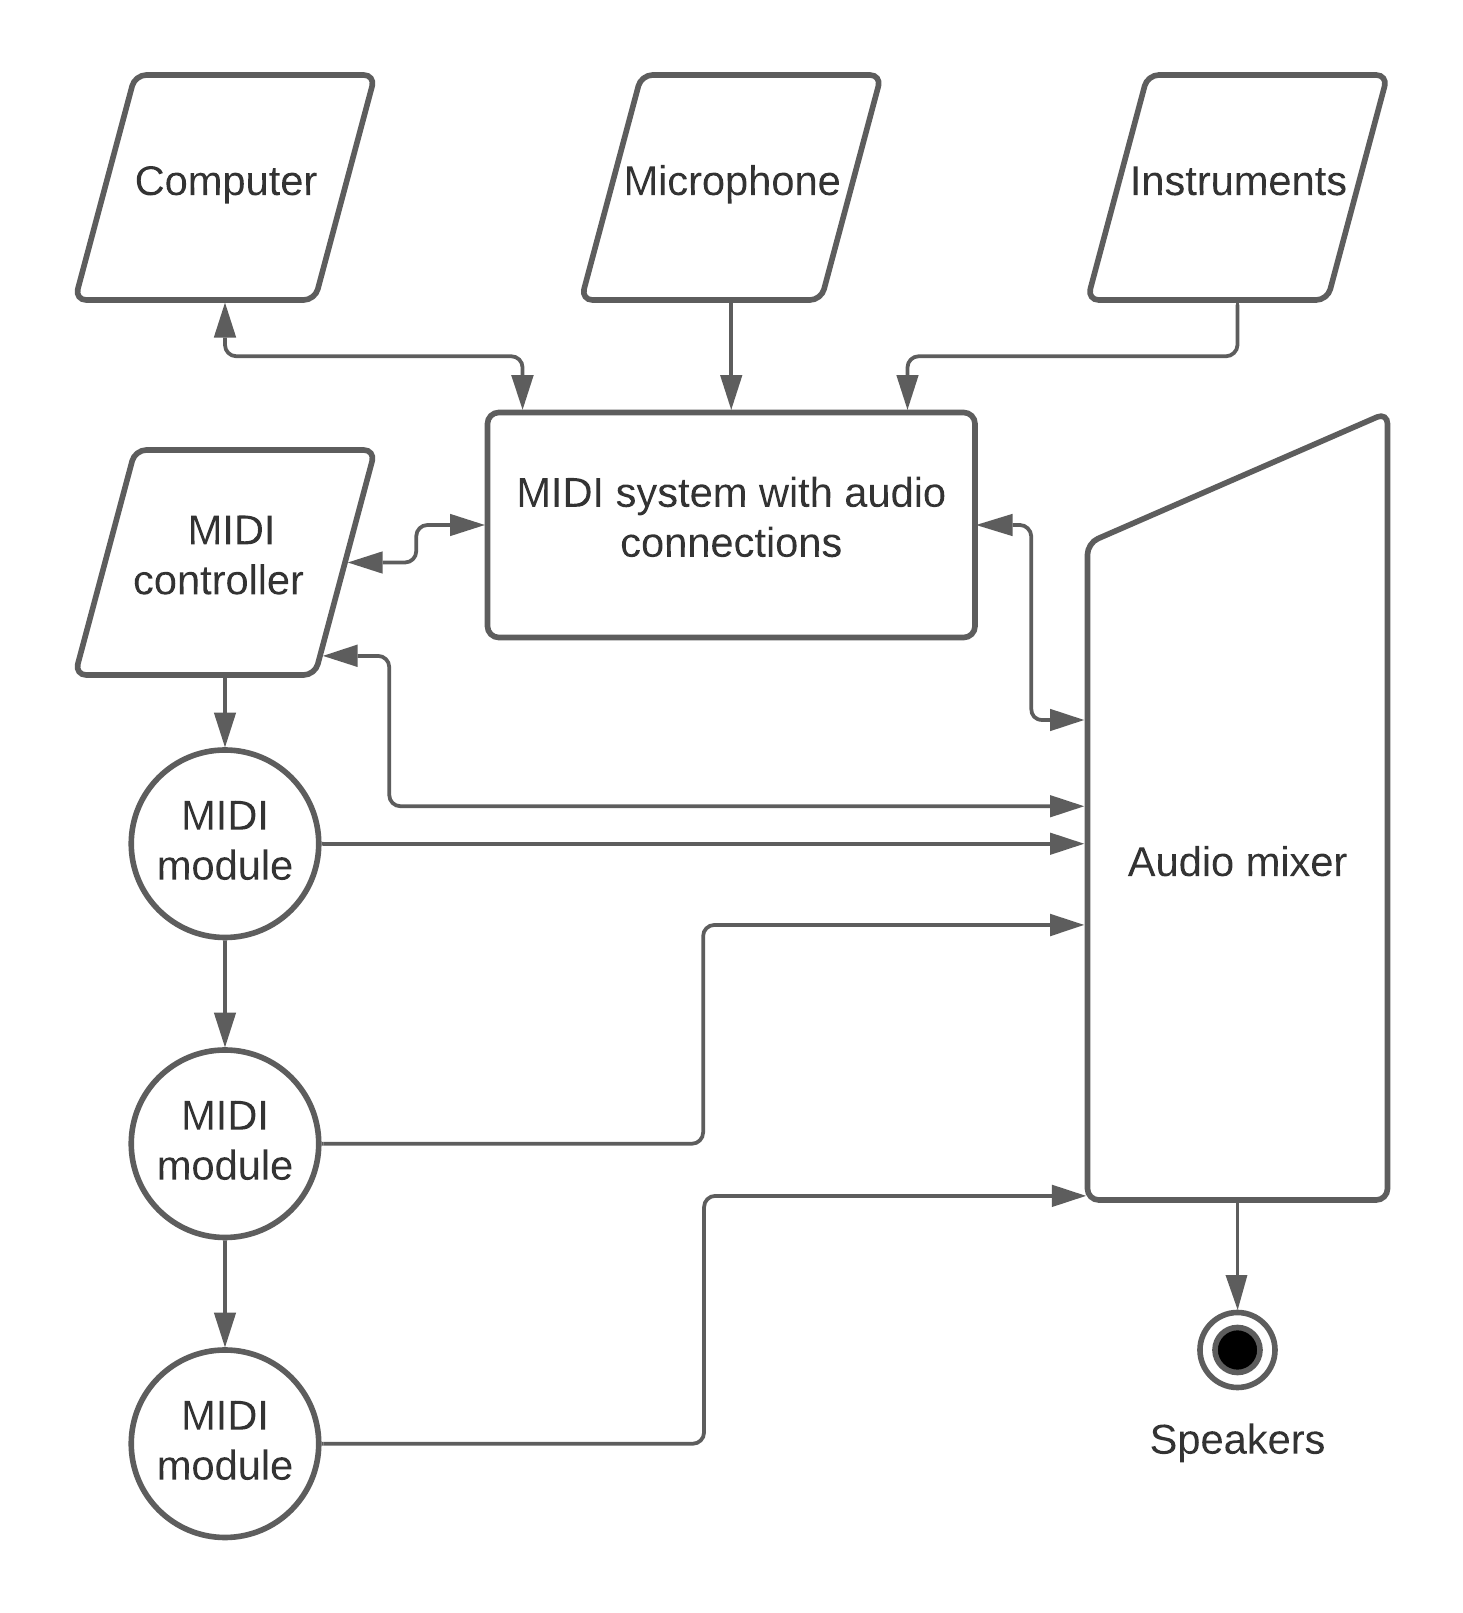
\includegraphics[width=0.35\textwidth]{figures/midi-system-with-audio-connections.png}
	\caption{The MIDI system, with audio connections}
	\label{fig:midi-system-with-audio-connections}
\end{figure}

Additionally, much of MIDI is built around the concept of keyboard notes and pitches. MIDI messages are primarily transmitted through the use of an electronic keyboard. So, for other types of MIDI instruments (such as a violin, or clarinet), there is a restriction to how a note may sound using MIDI. Certain characteristics of non-keyboard instruments (such as the ability of playing discrete semitone pitches) are more easily lost. For players of acoustic instruments, these issues are even more clear. Within MIDI, the velocity considered to be a single note-on velocity, defining the dynamic response of the note to one value. For players of acoustic instruments, the velocity, or dynamic response, of a singular note is shaped by the player, along with the note's timbre and pitch when played\cite{Kirk_Hunt_2013}.

\subsection[How does MIDI work?]{How does MIDI work?}\label{section:how-midi}

A MIDI receiver will receive MIDI messages that contain information about musical notes or events. These MIDI messages, or commands, are communicated through one of MIDI's 16 channels, numbered one through sixteen. These musical messages include information about a note's notation, pitch, velocity\footnote{This is typically a note's volume or loudness.}, vibrato, panning information\footnote{Whether a note is panned to the right or the left of stereo.}, and clock signals\footnote{These set the tempo of a note.}, among others.\footnote{Further reading can be found in Romano 2003, which discusses several other important MIDI commands, such as note on, note off, and aftertouch.} MIDI itself does not produce sound or music, but the instructions for a MIDI receiver include which sounds to play. These instructions are given in binary, combined into byte-sized commands. The protocol itself provides support for 128 notes, which ranges from C five octaves below middle C (or $C_0$) up to $G_{10}$ (ten octaves higher).